% sesmesh — Solvent Excluded Surface meshes for molecules
% Copyright (c) 2026 Ugo Varetto
% SPDX-License-Identifier: MIT OR Apache-2.0

\section{Introduction}
\label{sec:intro}

\paragraph{Molecular surfaces.}
A molecule is commonly modelled as a union of balls, one per atom, with van
der Waals (vdW) radii; the solvent is modelled as a spherical probe, by
convention of radius $r_p = 1.4$\Ang{} for water. Three surfaces follow from
this model. The \emph{vdW surface} is the boundary of the union of the atom
balls. The \emph{solvent-accessible surface} (SAS) of Lee and
Richards~\cite{lee1971} is the locus of the probe \emph{centre} as it rolls
over the molecule, i.e.\ the boundary of the union of balls with radii
grown by $r_p$. The \emph{solvent-excluded surface} (SES), also called the
molecular or Connolly surface, is the locus of the inward-facing probe
\emph{surface}: the boundary of the region that no probe ball can enter
without overlapping an atom~\cite{richards1977,greer1978,connolly1983jac,connolly1983science}.
The SES is smooth almost everywhere and consists of three kinds of
patches~\cite{connolly1983jac}: convex spherical patches where the probe
touches one atom, toroidal (saddle) patches swept while it touches two, and
concave spherical triangles where it touches three
(\cref{fig:gallery-kinds}). It is widely used to visualize
macromolecules~\cite{kozlikova2017}, to measure their area, volume and
internal cavities, and as the dielectric boundary in continuum
electrostatics, where boundary- and finite-element solvers need a closed,
manifold triangulation \todo{cite representative Poisson--Boltzmann BEM/FEM
solvers that consume SES meshes; none is in the repository's reference
list}.

\paragraph{Existing programs.}
Two families of programs triangulate the SES. \emph{Analytic} methods
compute every probe placement and patch boundary exactly and then
triangulate the patches: Connolly's original program~\cite{connolly1983jac},
the reduced surface of MSMS~\cite{sanner1996}, the contour-buildup
algorithm~\cite{totrov1996,lindow2010} and the template meshing of Quan and
Stamm~\cite{quan2017}; sesa computes analytic SES
areas~\cite{wang2024sesa}. They give exact geometry and compact,
well-shaped meshes, but the SES has singularities---self-intersecting tori
where the probe cannot pass between two atoms, and intersecting concave
patches where probe placements overlap---which make patch construction
numerically delicate~\cite{quan2016}. MSMS restarts a failing computation
up to five times after enlarging the radii of the atoms involved by
0.1\Ang~\cite{msmsmanual}; Goddard found that it crashed on most structures
larger than 10\,000 atoms~\cite{goddard2013}, and Decherchi and Rocchia
report that it fails to detect the internal cavity of a
fullerene~\cite{decherchi2013}. MSMS is distributed under a licence that is
not open source~\cite{msmsmanual}.

\emph{Volumetric} methods sample a function on a grid and extract an
isosurface. EDTSurf~\cite{xu2009edtsurf} voxelizes the SAS, computes a
Euclidean distance transform~\cite{felzenszwalb2012,maurer2003} and
thresholds it at $r_p$; related approaches use level
sets~\cite{can2006lsms}, Eulerian formulations~\cite{liu2017eses} or a
distance grid as in UCSF Chimera and ChimeraX, whose surface command
exposes essentially a single quality setting, the grid spacing
(default 0.5\Ang)~\cite{goddard2013,chimeraxsurface}. Grid methods are
robust and make resolution an explicit parameter, but their distances are
approximate: Xu and Zhang report area and volume errors of 3.96\,\% and
1.18\,\% at a $128^3$ grid, and 1.99\,\% and 0.48\,\% at $256^3$, relative
to MSMS~\cite{xu2009edtsurf}. NanoShaper~\cite{decherchi2013} combines both
families: it builds the analytic patches (with CGAL alpha shapes), casts
rays along grid lines, intersects them exactly with the patches and
triangulates the result with Marching Cubes tables, so its vertices lie on
the surface. On GPUs, Hermosilla et al.~\cite{hermosilla2017} and
QuickSES~\cite{martinez2019quickses} compute narrow-band distance grids
organized in bricks; Hermosilla et al.\ report about 1.65\,s for the
545\,000-atom 1K4R capsid on a $512^3$ grid (GeForce GTX 970), with
distances approximated grid point to grid point. Finally, the SES can be
written as a level set of an implicit
function~\cite{parulek2012,quan2016}: Quan and Stamm proved that it is
exactly the $r_p$-level set of the distance to the SAS, computable from
three classes of closest features~\cite{quan2016}.

\paragraph{Failure modes.}
Our own comparison of current versions on the same spheres
(\cref{sec:comparison}) shows four recurring problems.
(i)~\emph{Failures}: MSMS stopped with an error on several large or
irregular structures even after its restarts, NanoShaper crashed or stopped
on a large ribosome at a fine grid, on a 2.4-million-atom capsid and on one-
and two-atom inputs, EDTSurf aborted on both 1\Ang{} capsids, and ESES
crashed on coordinates far from the origin.
(ii)~\emph{Meshes that are not closed 2-manifolds or not on the surface}:
many MSMS meshes have non-manifold edges and vertices up to several \AA{}
from the SES, ChimeraX writes each patch with separate vertices, and
NanoShaper occasionally places vertices far from the surface.
(iii)~\emph{Accuracy tied to the voxel size} in grid-distance
methods~\cite{xu2009edtsurf}: ChimeraX's surface area is several per cent
low at its default spacing, and dense grids need memory that grows with the
volume of the bounding box rather than with the surface area.
(iv)~\emph{Results that depend on the run}: ESES's mesh changed with the
number of threads; reproducible meshes matter for regression testing,
caching and published supplementary data.
To our knowledge no Rust library computes SES meshes; existing Rust crates
in this area compute numerical solvent-accessible surface
areas~\cite{rustsasa}.

\paragraph{This work.}
\sesmesh{} combines the exact implicit characterization of Quan and
Stamm~\cite{quan2016} with the sparse narrow-band bricks of GPU
methods~\cite{hermosilla2017,museth2013}, the exact edge intersections of
NanoShaper~\cite{decherchi2013} and Marching Cubes~\cite{lorensen1987}, in a
dependency-light, multi-threaded and vectorized CPU implementation. Its
contributions are:
\begin{enumerate}
  \item a narrow-band sampling of the exact SES field on a sparse brick
    lattice, with conservative culling based on the 1-Lipschitz property of
    the field, so that time and memory scale with the surface, not the
    volume (\cref{sec:arrangement,sec:lattice});
  \item a Marching Cubes table with a uniform face-ambiguity rule, generated
    and verified exhaustively, which together with a single sign rule gives
    closed, consistently oriented, edge-manifold meshes that are validated
    before they are returned (\cref{sec:mc});
  \item exact vertex refinement and analytic normals, patch types and
    nearest atoms for every vertex, exact cavity classification by signed
    volume, and the identification of sub-grid fragments
    (\cref{sec:refine,sec:cavities,sec:fragments});
  \item level-of-detail controls that keep vertices on the exact surface:
    a calibrated vertex density, Taubin smoothing with exact re-projection,
    and quadric-error decimation by half-edge collapses (\cref{sec:lod});
  \item deterministic parallelism---byte-identical output for any thread
    count---with runtime SIMD dispatch, and a memory guard that predicts
    peak memory and can coarsen the grid to fit a limit
    (\cref{sec:implementation});
  \item a validation against analytic references, a \val{corpus-n}-entry
    accuracy study, a \val{sweep-n}-entry robustness sweep and inputs of up
    to 2.44 million atoms (\cref{sec:validation,sec:performance}), and a
    comparison on the same spheres with MSMS, NanoShaper, ESES, EDTSurf,
    ChimeraX and sesa (\cref{sec:comparison}).
\end{enumerate}
\sesmesh{} is a library first: the command-line tool is a thin layer over
a public Rust API that takes spheres and returns a mesh.

\Cref{sec:background} recalls the definitions and the implicit field;
\cref{sec:method} describes the algorithm and \cref{sec:implementation} its
implementation. \Cref{sec:validation,sec:performance} report accuracy,
robustness and performance; \cref{sec:comparison} compares \sesmesh{} with
other programs; \cref{sec:discussion}
discusses limitations, and \cref{sec:availability} gives availability.

\begin{figure}[t]
  \centering
  \begin{subfigure}[b]{0.32\linewidth}
    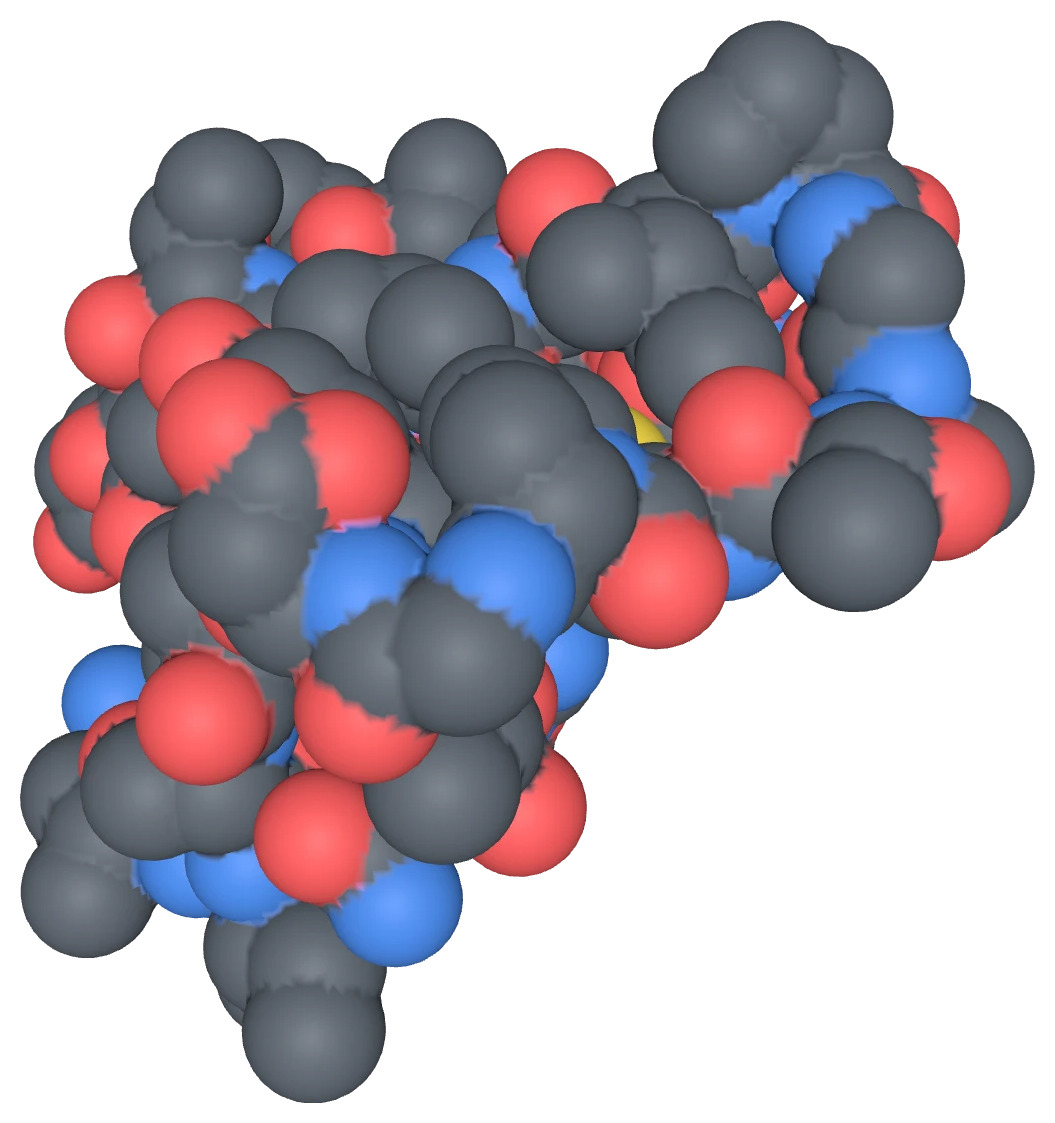
\includegraphics[width=\linewidth]{1crn-vdw}
    \caption{vdW surface}
  \end{subfigure}\hfill
  \begin{subfigure}[b]{0.32\linewidth}
    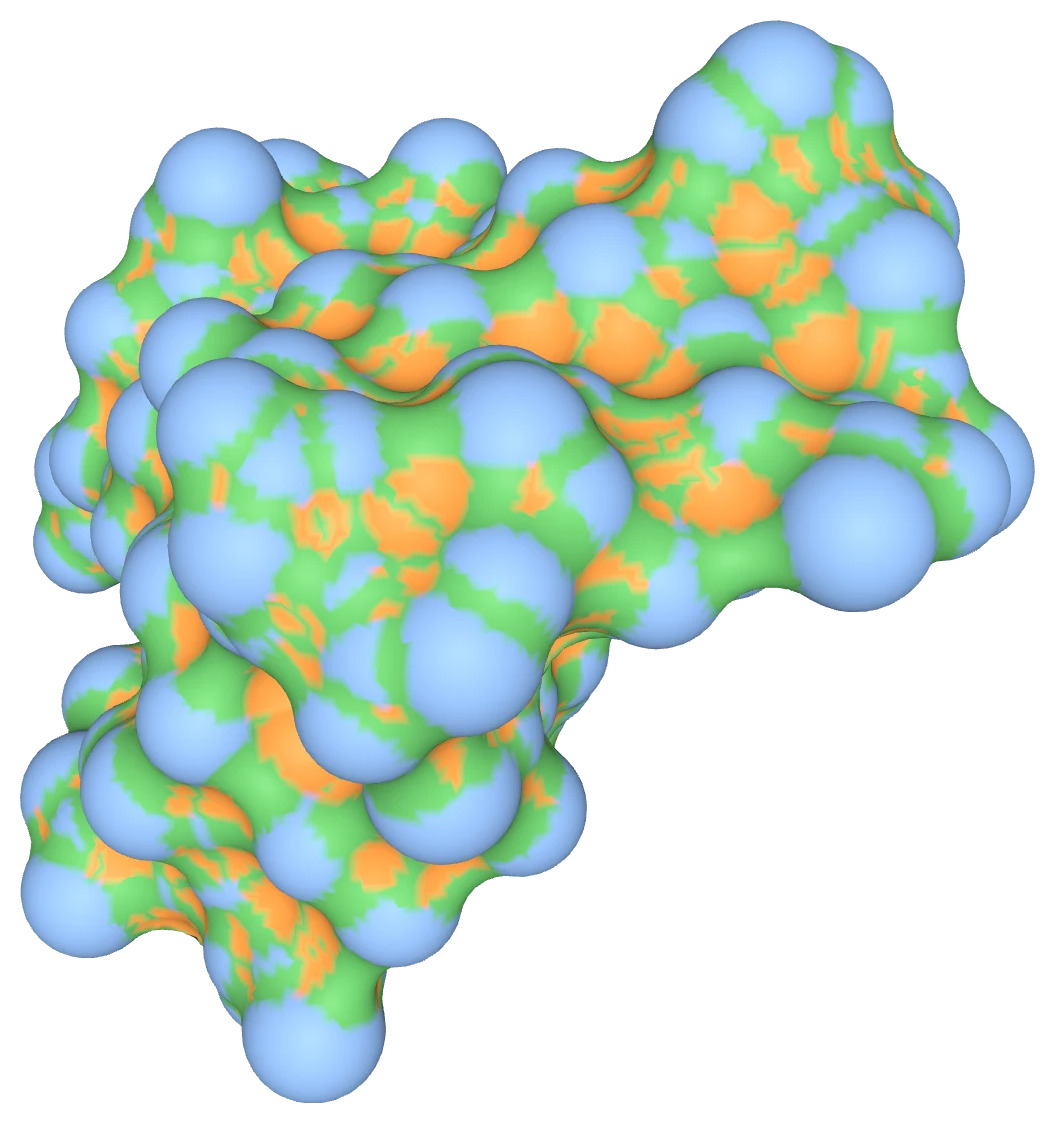
\includegraphics[width=\linewidth]{1crn-patch}
    \caption{SES, by patch type}
  \end{subfigure}\hfill
  \begin{subfigure}[b]{0.32\linewidth}
    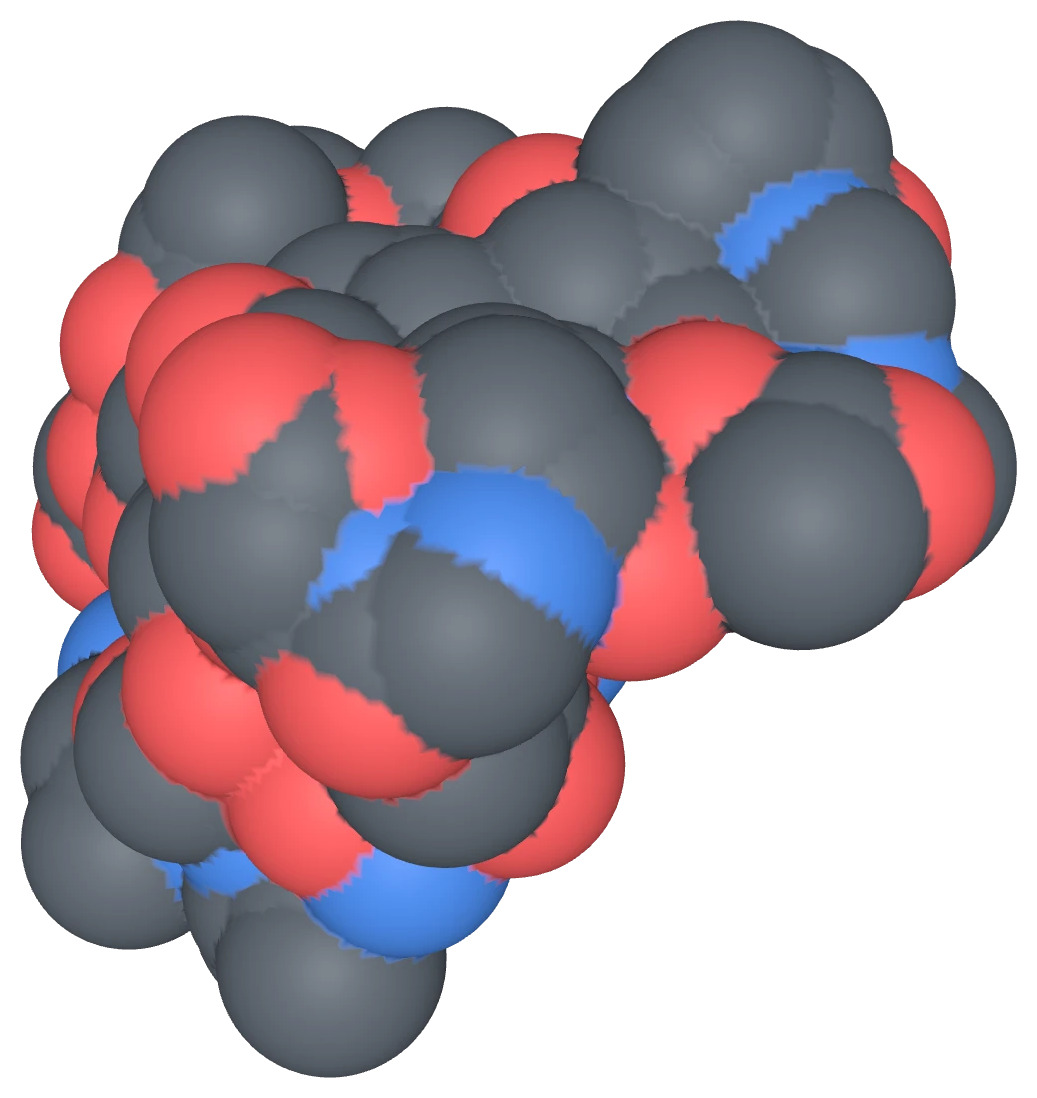
\includegraphics[width=\linewidth]{1crn-sas}
    \caption{SAS}
  \end{subfigure}
  \caption{The three surfaces of crambin (PDB 1CRN, 327 atoms) computed by
    \sesmesh{} at $h = 0.25$\Ang. (a)~vdW surface, coloured by element
    (198\,268 triangles). (b)~SES coloured by the patch type of each vertex:
    convex (blue), saddle (green), concave (orange). (c)~SAS, atom radii
    grown by $r_p = 1.4$\Ang. Renderings from the project website.}
  \label{fig:gallery-kinds}
\end{figure}
